\documentclass[dvipsnames, format=sigconf]{acmart}


\acmDOI{10.1145/nnnnnnn.nnnnnnn} % To be updated after completing copyright process
\acmISBN{978-x-xxxx-xxxx-x/YY/MM} % To be updated after completing copyright process
\acmConference[GECCO '24]{The Genetic and Evolutionary Computation Conference 2024}{July 14--18, 2024}{Melbourne, Australia}
\acmYear{2024}
\copyrightyear{2024}

%%
%% The majority of ACM publications use numbered citations and
%% references.  The command \citestyle{authoryear} switches to the
%% "author year" style.
%%
%% If you are preparing content for an event
%% sponsored by ACM SIGGRAPH, you must use the "author year" style of
%% citations and references.
%% Uncommenting
%% the next command will enable that style.
%%\citestyle{acmauthoryear}


% \usepackage[utf8]{inputenc} % allow utf-8 input
% \usepackage[T1]{fontenc}    % use 8-bit T1 fonts

% \usepackage{amsfonts}       % blackboard math symbols
% \usepackage{amsmath}
% \usepackage{amsthm}
% \theoremstyle{definition}
% \newtheorem{definition}{Definition}

\usepackage{booktabs}       % professional-quality tables
\usepackage{tabularx}
\usepackage{graphicx}
\usepackage{subcaption}
\usepackage{color}
\usepackage{qrcode}


% \PassOptionsToPackage{hyphens}{url} % url is loaded by hyperref
\usepackage{hyperref}
\renewcommand{\sectionautorefname}{Section}
\renewcommand{\subsectionautorefname}{Section}
\renewcommand{\subsubsectionautorefname}{Section}
\newcommand{\definitionautorefname}{Definition}

\usepackage{xspace}
\newcommand{\eg}{e.g.,\xspace}
\newcommand{\ie}{i.e.,\xspace}
\newcommand{\cf}{cf.,\xspace}

% \usepackage{adjustbox}
% \usepackage{wrapfig}
% \usepackage{caption,subcaption}

\newcommand{\achiya}[1]{{\textcolor{red}{[Achiya: #1]}}}
\newcommand{\irina}[1]{{\textcolor{blue}{[Achiya: #1]}}}

\usepackage{listings}
\usepackage{ulem}
%\usepackage{multirow}
%\usepackage{titlesec}

\lstset{
    escapeinside={!}{!},
    language=[x86masm]Assembler,
    basicstyle=\scriptsize,
    keywordstyle=\bfseries,
    commentstyle=\itshape,
    numbers=left,
    numberstyle=\tiny,
    numbersep=6pt, 
    frame=lines,
    breaklines=true
}
\AtBeginDocument{\DeclareCaptionSubType{lstlisting}}
\newcommand{\lstin}[2][]{\lstinline[#1]|#2|}

\usepackage{framed}
\newenvironment{BNF}
  {\captionsetup{type=lstlisting}}
  {}
\usepackage[nounderscore]{syntax}
\setlength{\grammarparsep}{0.1cm}
\setlength{\grammarindent}{2em}

\usepackage[para,flushleft]{threeparttable}

\newcolumntype{L}[1]{>{\raggedright\let\newline\\\arraybackslash\hspace{0pt}}m{#1}}
\newcolumntype{C}[1]{>{\centering\let\newline\\\arraybackslash\hspace{0pt}}m{#1}}
\newcolumntype{R}[1]{>{\raggedleft\let\newline\\\arraybackslash\hspace{0pt}}m{#1}}



\usepackage{multirow}
\usepackage{dblfloatfix}
\usepackage{balance} 


\begin{document}
%% Title
\title{Evolving Assembly Code in an Adversarial Environment}
%Assembly code evolution for CodeGuru players
%%%% Cite as
%%%% Update your official citation here when published 
% \thanks{\textit{\underline{Citation}}: 
% \textbf{Authors. Title. Pages.... DOI:000000/11111.}} 
%}

\author{Irina Maliukov}
\email{irinamal@post.bgu.ac.il}
\orcid{0009-0006-9300-5397}
\author{Gera Weiss}
\email{geraw@bgu.ac.il}
\orcid{0000-0002-5832-8768}
\author{Oded Margalit}
\email{odedm@post.bgu.ac.il}
\orcid{0000-0002-2026-2601}
\affiliation{%
  \institution{Department of Computer Science\\Ben-Gurion University of the Negev}
  \city{Be'er Sheva}
  \country{Israel}
}

\author{Achiya Elyasaf}
\email{achiya@bgu.ac.il}
\orcid{0000-0002-4009-5353}
\affiliation{%
  \institution{Department of Software and Information System Engineering\\Ben-Gurion University of the Negev}
  \city{Be'er Sheva}
  \country{Israel}
}

\renewcommand{\shortauthors}{Maliukov et al.}

\begin{abstract}
In this work, we evolve assembly code for the CodeGuru competition. The goal is to create a survivor---an assembly program that runs the longest in shared memory, by resisting attacks from adversary survivors and finding their weaknesses.
For evolving top-notch solvers, we specify a \textit{Backus Normal Form} (BNF) for the assembly language and synthesize the code from scratch using \textit{Genetic Programming} (GP). We evaluate the survivors by running CodeGuru games against human-written winning survivors. 
Our evolved programs found weaknesses in the programs they were trained against and utilized them.
%In addition, we compare our approach with a Large-Language Model, demonstrating that the latter cannot generate a survivor that can win at any competition. 
This work has important applications for cyber-security, as we utilize evolution to detect weaknesses in survivors. The assembly BNF is domain-independent; thus, by modifying the fitness function, it can detect code weaknesses and help fix them. 
Finally, the CodeGuru competition offers a novel platform for analyzing GP and code evolution in adversarial environments. To support further research in this direction, we provide a thorough qualitative analysis of the evolved survivors and the weaknesses found.
\end{abstract}

%%
%% The code below is generated by the tool at http://dl.acm.org/ccs.cfm.
%% Please copy and paste the code instead of the example below.
%%
\begin{CCSXML}
<ccs2012>
   <concept>
       <concept_id>10011007.10011006.10011008.10011009.10011020</concept_id>
       <concept_desc>Software and its engineering~Assembly languages</concept_desc>
       <concept_significance>500</concept_significance>
       </concept>
   <concept>
       <concept_id>10011007.10011074.10011092.10011782.10011813</concept_id>
       <concept_desc>Software and its engineering~Genetic programming</concept_desc>
       <concept_significance>500</concept_significance>
       </concept>
   <concept>
       <concept_id>10011007.10011006.10011041.10011047</concept_id>
       <concept_desc>Software and its engineering~Source code generation</concept_desc>
       <concept_significance>500</concept_significance>
       </concept>
   <concept>
       <concept_id>10011007.10011074.10011784</concept_id>
       <concept_desc>Software and its engineering~Search-based software engineering</concept_desc>
       <concept_significance>300</concept_significance>
       </concept>
   <concept>
       <concept_id>10002978.10003006.10011634</concept_id>
       <concept_desc>Security and privacy~Vulnerability management</concept_desc>
       <concept_significance>300</concept_significance>
       </concept>
   <concept>
       <concept_id>10010147.10010257.10010293.10011809.10011813</concept_id>
       <concept_desc>Computing methodologies~Genetic programming</concept_desc>
       <concept_significance>500</concept_significance>
       </concept>
 </ccs2012>
\end{CCSXML}

\ccsdesc[500]{Software and its engineering~Assembly languages}
\ccsdesc[500]{Software and its engineering~Genetic programming}
\ccsdesc[500]{Software and its engineering~Source code generation}
\ccsdesc[300]{Software and its engineering~Search-based software engineering}
\ccsdesc[300]{Security and privacy~Vulnerability management}
\ccsdesc[500]{Computing methodologies~Genetic programming}

%%
%% Keywords. The author(s) should pick words that accurately describe
%% the work being presented. Separate the keywords with commas.
\keywords{genetic programming, assembly, code generation, cyber-security, CodeGuru Xtreme}

%% A "teaser" image appears between the author and affiliation
%% information and the body of the document, and typically spans the
%% page.
% \begin{teaserfigure}
%   \includegraphics[width=\textwidth]{sampleteaser}
%   \caption{Seattle Mariners at Spring Training, 2010.}
%   \Description{Enjoying the baseball game from the third-base
%   seats. Ichiro Suzuki preparing to bat.}
%   \label{fig:teaser}
% \end{teaserfigure}

%%
%% This command processes the author and affiliation and title
%% information and builds the first part of the formatted document.
\maketitle

\section{Introduction}
CodeGuru Xtreme~\cite{codeguru_repo} is a coding competition where short 8086 assembly programs, called survivors, are loaded into a random address in a virtual computer memory arena. Their goal is to defeat all other survivors by staying the last program to run. An opponent is defeated when it runs an illegal command caused, \eg by overwriting its memory. The screen-shot of the game screen is depicted in \autoref{fig:CodeGuru}. Each survivor gets a different color in the arena, representing the bytes it wrote to the shared memory. We elaborate on the game in \autoref{sec:codeguru}.

\begin{figure}
  \centering
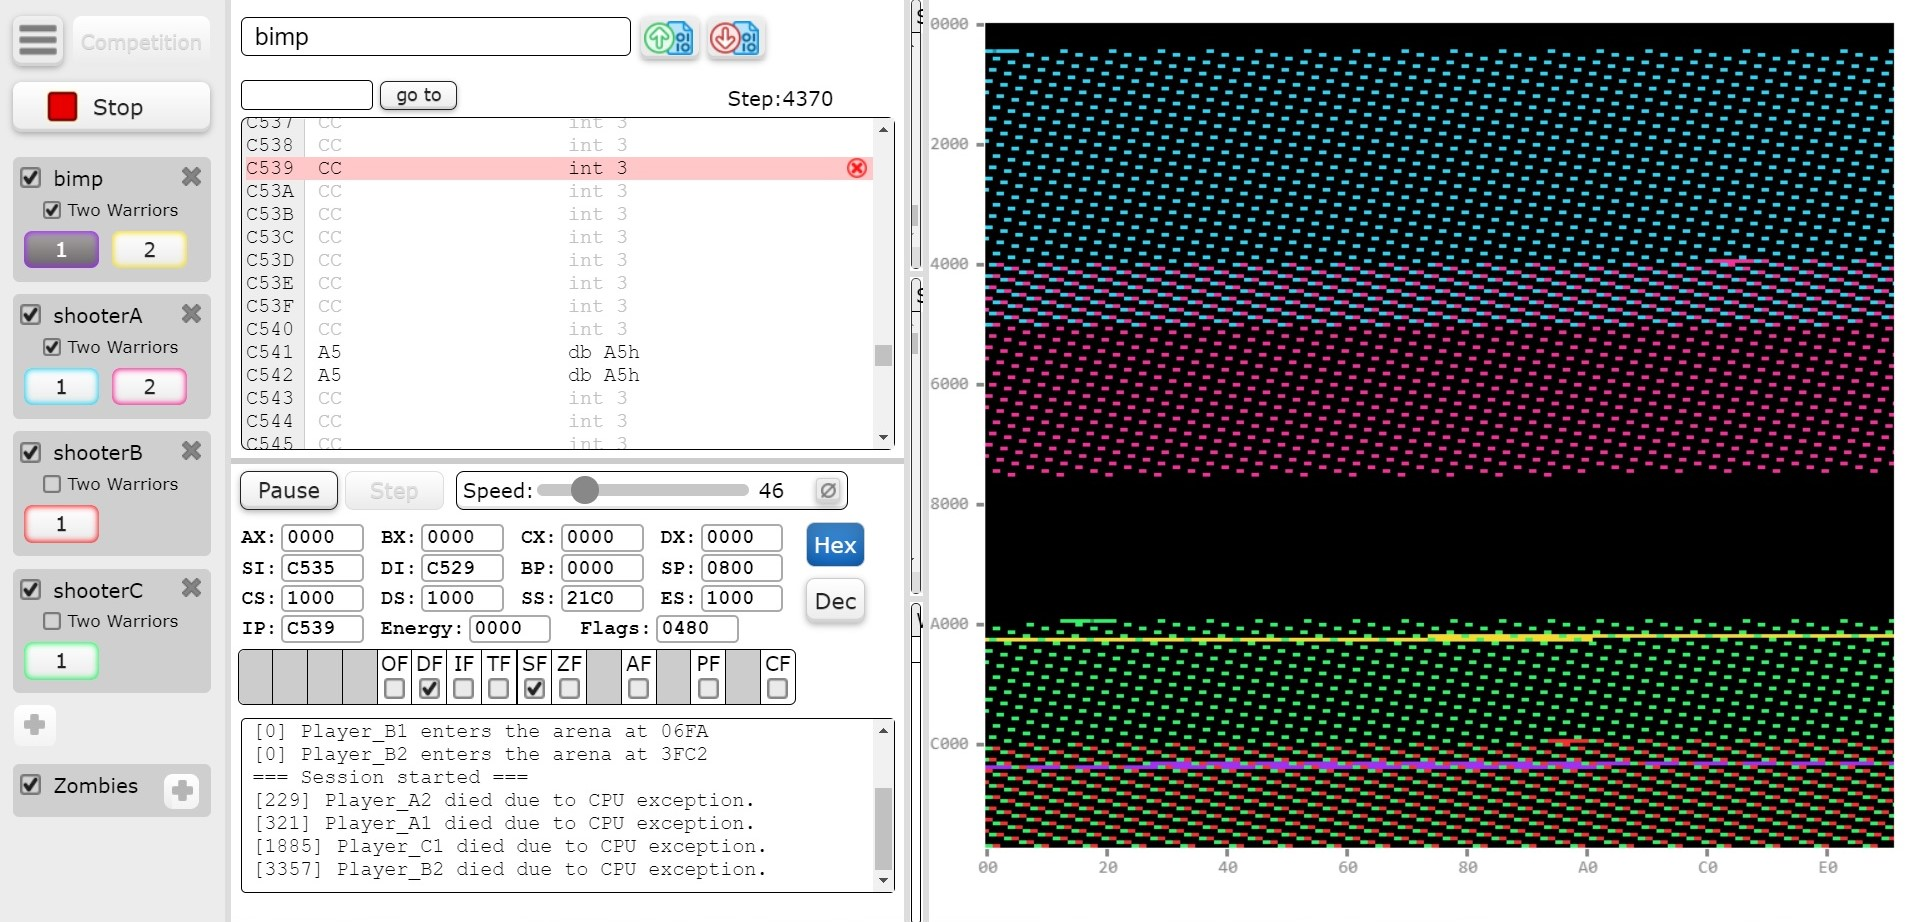
\includegraphics[width=\linewidth]{images/memory_use.jpg} 
  \caption{The CodeGuru Xtreme game. On the left are the survivors; on the center is the code of the selected survivor; and on the right is the arena, \ie the memory status. Each survivor gets a different color in the arena, representing the bytes it wrote to the shared memory.}
  \label{fig:CodeGuru}
  \Description{Capture of the CodeGuru Xtreme game. On the left are the survivors; on the center is the code of the selected survivor; and on the right is the arena, \ie the memory status. Each survivor gets a different color in the arena, representing the bytes it wrote to the shared memory.}
\end{figure}

In this work, we evolve winning survivors from scratch, \ie from randomly generated assembly code, and without access to the source code of known survivors. For this task, we utilize \textit{Grammar-Guided Genetic Programming} (G3P)---an evolutionary computation technique that incorporates GP principles, employs context-free grammar and operates directly with tree-based representations. G3P allows us to evolve assembly programs following grammar-type constraints. The goal of the individuals, embodied by the fitness function, is to overtake adversaries and win the game. The evolved code is represented using an \textit{Abstract Syntax Tree} (AST) based on matching assembly BNF we defined, where the nodes and leaves are the BNF's functions and terminals, respectively. Since our BNF and the operators we used are general and domain-agnostic, the approach applies to generating assembly programs for other domains and processors.

% CodeGuru Xtreme~\cite{codeguru_repo} is a coding competition based on ``Core War''---a 1984 programming game created by D. G. Jones and A. K. Dewdney~\cite{dewdney1984recreational}.

No previous work has been done on the CodeGuru Xtreme game, except for an undergraduate project~\cite{Darwin8086} and some early work on the ``Core War'' game~\cite{Andersen2001TheGE, corno2003exploiting}, which served as the basis for CodeGuru Xtreme (see \autoref{sec:codeguru}). As elaborated in \autoref{sec:related-work}, some work has been done on the evolution of low-level languages (\ie assembly and Java bytecode), and some work has been done %utilized large-language models (LLM)
to improve existing assembly code. Note that improving existing code is a simpler task than generating new code from scratch, as the former's state space is much smaller~\cite{Petke2018GeneticImprovementSoftware, Banzhaf2018SomeRemarksCode}. %To support that, we compared our approach to using LLM in \autoref{sec:llm}, demonstrating that the latter fails to create a survivor that wins any competition, even when playing against simple survivors.

%AEAE this should go to the method section where we talk about why we chose G3P
% Previous attempts to evolve low-level programs have focused Grammatical Evolution (GE), code synthesis, Multi-objective Linear Genetic Programming (MOLGP), Grammar-Guided Genetic Programming (G3P) and PushGP. We chose to use G3P based on typed tree-GP over the others due to the convenience of using BNF for assembly language in the evolution and being able to perform direct changes on the evolved tree program. The fact that PushGP is based on type stacks and type matching operators makes it harder to adjust to assembly code and other approaches, as MOLGP, weren't fully applied to unrestricted assembly language.

CodeGuru Xtreme competition has been running since 2005, with all past survivors publicly available. Thus, winning is considerably tricky and requires, among other qualities, a good understanding of the 8086 assembly language. %We will show that generating top-notch survivors that outtake past survivors is a challenging  task. 

% --->
This work has implications for cyber-security. As demonstrated below, we utilize evolution to detect and exploit weaknesses in other survivors. In addition, understanding the assembly language is a necessity in some viruses. By modifying the fitness function, our approach can be used for detecting weaknesses in code and help in fixing them, detecting suspicious adversarial code, or, on the contrary, can be intended to avoid security mechanisms by mutating the virus to avoid detection while keeping its functionality. Finally, our approach can evolve high-quality individuals with a small number of examples and without detailed information. 

The CodeGuru Xtreme competition provides a unique opportunity to analyze \textit{Genetic Programming} (GP) and code evolution in adversarial environments. In order to encourage further research in this area, we conducted a comprehensive qualitative analysis of the evolved survivors and identified their strengths and weaknesses. This analysis sheds light on the effectiveness of the evolved code and provides valuable insights for future improvements and advancements in the field.

\section{Related Work}
\label{sec:related-work}
\paragraph{Low-level code evolution}
Several works have been done on low-level code evolution, some similar to assembly, like Verilog (a hardware description language) and Java bytecode. Karpuzcu~\cite{ulya2005automatic} used Grammatical Evolution (GE) for evolving a simple program of a one-bit full adder. %They created BNF for the subset of Verilog syntax used in this example and forced assignments to proper expressions and limited nested statements. 
In spite of the strong bias they employed, the success achieved was only about 5.7\%. 

Orlov and Sipper~\cite{orlov2011flight} proposed a method for genetic improvement and repair of existing Java programs or any software that can be compiled into Java bytecode. Although Java bytecode resembles assembly, it has a simplified representation and does not have direct memory access. This contrasts assembly, which has very strong correspondence between its instructions, the architecture's machine code instructions, and memory. %The authors created a novel crossover, which ensures a viable bytecode offspring (that compiles without error) by holding some conditions on JVM's operand stack, local variables, and control flow. Since assembly does not have a stack-based architecture like JVM for its execution, we will ensure viable assembly offspring using type constraints. Notably, 
Orlov and Sipper seeded the initial population with copies of a single hand-crafted individual and improved it over generations, while we evolve assembly code from scratch.

Rosin~\cite{Rosin2019Stepping} synthesized simple programs with loops from input/output examples. They targeted simplified low-level language similar to assembly, where each instruction consists of an opcode and a single operand. %Rosin used delayed acceptance hill-climbing, which, instead of immediately accepting an update to the current-best candidate solution, continues to gather additional candidates for $n$ steps and then accepts the best found during that period. This is done to avoid local optimums. 
% They compared their results with TIS-100, an assembly language programming game for players who tracked the best programs they could find for each puzzle. One of the categories is to minimize the number of instructions and the generated code matched the best reported program.
% Their results show that synthesized assembly-like programs can compete with human-written ones. We want to expend this approach by evolving assembly code from scratch, worthy to over take human-written code.

% They do not use the approach in genetic programming that involves definition of functions and terminals appropriate to the problem. They use evolution of machine code to repair human-written programs. 

\paragraph{Limited assembly code evolution}
Some works focused on constrained assembly evolution---specific routines, predefined input and output tables, and manually written code parts.
In \cite{Serruto2017Automatic}, multi-objective linear genetic programming is applied for the automatic generation of some specific assembly driver routines. %For fitness evaluation, they maximize a function to each bit of the binary result or the timing diagram of each used micro-controller Port pins, respectively to the targeted routine. 
The architecture used was an 8051 microcontroller assembly, which is similar to the 8086 we use. The evolved programs did not contain jump instructions because they could form infinite loops, in contrast to our wish to include them in the generated code. %They adopted LGP chromosome representation with dynamic size because in the evolutionary process instructions of micro-controller program are in machine language, which is an imperative language. They tested their results using two multi-objective optimization algorithms: EMOEA and NSGAII and compared them to written-by-human programs taken from micro-controller assembly language programming courses. 
The results showed that the automatically generated microcontroller code for specific tasks can compete with a human programmer with a smaller code size or faster execution. We aim to recreate this result within an adversarial environment.

Similarly, \cite{Ferrel2020Genetic} presented a methodology for writing Arduino board programs using an automatic generator of assembly language routines based on a cooperative co-evolutionary multi-objective linear genetic programming algorithm. They decomposed the problem into sub-components, generating about 73\% of the program, and the remaining 27\%, which are the main program and initial configuration routines, are manually written.% The automatic generation also requires an input-output table for the routine. Each generated routine corresponds to a pin of a Port or one bit of the objective code, depending its purpose. One of the pointed limitations of the proposed methodology is that the application of it depends on the existence of sub-tasks that are described by input-output tables.
In our case, we cannot break the goal of winning an opponent to sub-tasks without reading its code first, which we avoid. In addition, there is no clear way to represent a winning result in our case using an input-output table. We need to evolve from scratch, a winning program, including jumps and loops, completely automatically. The presented method~\cite{Ferrel2020Genetic} requires more general implementation and adaptations to match our use case, yet prove the ability to achieve it.


\paragraph{Overview of Program Synthesis Methods} 
Several articles compare recent program synthesis and evolution techniques.
\cite{Pantridge2017On} compares Flash Fill (Microsoft Excel feature which uses version-space algebras to perform program synthesis from examples on string manipulation tasks), MagicHaskeller (synthesizes functional Haskell programs with an exhaustive search of programs minimizing the search space using Monte-Carlo algorithm to remove semantically equivalent programs), TerpreT (a probabilistic programming language that is designed for inductive program synthesis), and two forms of GP---PushGP (evolves programs in a Turing complete, stack-based language called Push) and Grammar Guided Genetic Programming (a GP that uses context-free grammar as a guideline for syntactically correct programs throughout the evolution). The comparison focused on the possibility of producing a program that passes all tests for all training and unseen testing inputs. It was done on problems of two types: the first is usually approached using machine code or assembly language (basic execution models problems), while the second is usually approached using high-level languages (general program synthesis benchmark suite). In the low-level field, the system that performed the best was TerpreT, while sadly, there were no gathered results for G3P. In the high-level field, both GP approaches outperformed the others.

A survey of recent developments in program synthesis with evolutionary algorithms~\cite{domonik2021recent}, found that the most influential approaches in the field are stack-based GP (usually PushGP), G3P, and Linear GP (uses registers for calculations and direct memory access).
Encouraged by this review and by the fact that G3P has not been widely tested on low-level languages, we want to use G3P for the evolution of assembly programs.

%Google DeepMind created AlphaDev, a deep-reinforcement learning agent trained to improve a sorting algorithm~\cite{Mankowitz2023Faster}. They trained AlphaDev with up to 16 Tensor Processing Units (TPU) v.3, with a total batch size of 1,024 per TPU core and for 1 million iterations. In practice, across all tasks, training took them, in the worst case, two days to converge. Aside from the high resource demands for representing and training the neural network, their approach assumes a given working program to improve. It is not designed to create programs from scratch.

%A day after AlphaDev publication, a user on X (formerly Twitter) tried to use ChatGPT to optimize the same sorting algorithm~\cite{Papailiopoulos2023}. As noted before, improving an existing code is simpler than generating one from scratch. Nevertheless, we evaluate this approach in \autoref{sec:llm} and test whether it is applicable to our domain. 

All the related works present useful ideas for various research directions to achieve our goal of assembly code evolution. Yet, none achieved total success in evolving independent assembly programs from scratch. They all applied constraints and limitations on the programs, removed language features, or started from an initial given code. We aim to expand the above achievements. 

\section{CodeGuru}
\label{sec:codeguru}
CodeGuru Xtreme~\cite{codeguru_repo} is a coding competition based on ``Core War''---a 1984 programming game created by D. G. Jones and A. K. Dewdney~\cite{dewdney1984recreational}.
In CodeGuru Xtreme, short 8086 assembly programs (at most 512 bytes long) of 16-bit commands, called survivors, are loaded into random space on a virtual computer memory arena of size 64KB. Each survivor is loaded to a random address with a stack of 2,048 bytes and a full set of registers. The distance between two survivors and the arena's edges is at least 1,024 bytes.
The last survivor alive is the winner and gets one point. If several survivors stay alive, the point is divided equally between all.
A survivor is disqualified if it runs an illegal command or attempts to access a memory address outside the arena or its stack. A survivor can be forced to run an illegal command due to a writing operation an opponent previously performed on its code or on an address it reads from. Therefore, performing various writings to memory enhances the chance of damaging opponents, even silent opponents composed of sleep commands.
Each battle of the game runs for 200,000 rounds or until only one survivor is left, whichever comes first. In every round, the next command of each survivor is executed in a round-robin fashion. The order of the survivor's execution is changed randomly for each game. The memory arena image and scoreboard that monitors the game's progress are depicted in \autoref{fig:CodeGuru}. In most cases, each participant has two programs, called parts, that can collaborate together. Each part has its own registers and is loaded into a different place in memory, although they both share a stack. The parts are executed separately, one after the other. Their scores are joined together at the end of the battle and create the survivor's score. This allows to design of a survivor with two parts collaborating together via a shared stack or with two parts completely independently running, both designs are used as a force multiplier for maximizing the survivor's abilities. 
The game includes the following special commands: \texttt{WAITx4} increases the survivor's speed, allowing it to run several opcodes in a single round, \texttt{INT 0x86} writes 256 bytes into memory, and \texttt{INT 0x87} re-writes a pattern of 4 bytes. The special commands allow performing several rounds of actions in one round.  
% All of our experiments, were performed using survivors consisting of two programs.

CodeGuru competition has taken place every year since 2005 among outstanding high-school students. Each year, the level rises, with more sophisticated survivors written.
This work aims to evolve survivors that will win the top survivors of previous years by finding their weaknesses. Our goal is not to win the competition but rather to show that GP can be utilized for evolving code in an adversarial environment. Thus, we evolve a different survivor for each past survivor rather than evolving one survivor that takes them all.

% \begin{figure}
%   \centering
%   \begin{subfigure}{0.4\textwidth}
%     \includegraphics[width=\linewidth]{images/score_board.jpg}
%     \caption{Score board}
%     \label{fig:image1}
%   \end{subfigure}
%   \hfill
%   \begin{subfigure}{0.4\textwidth}
%     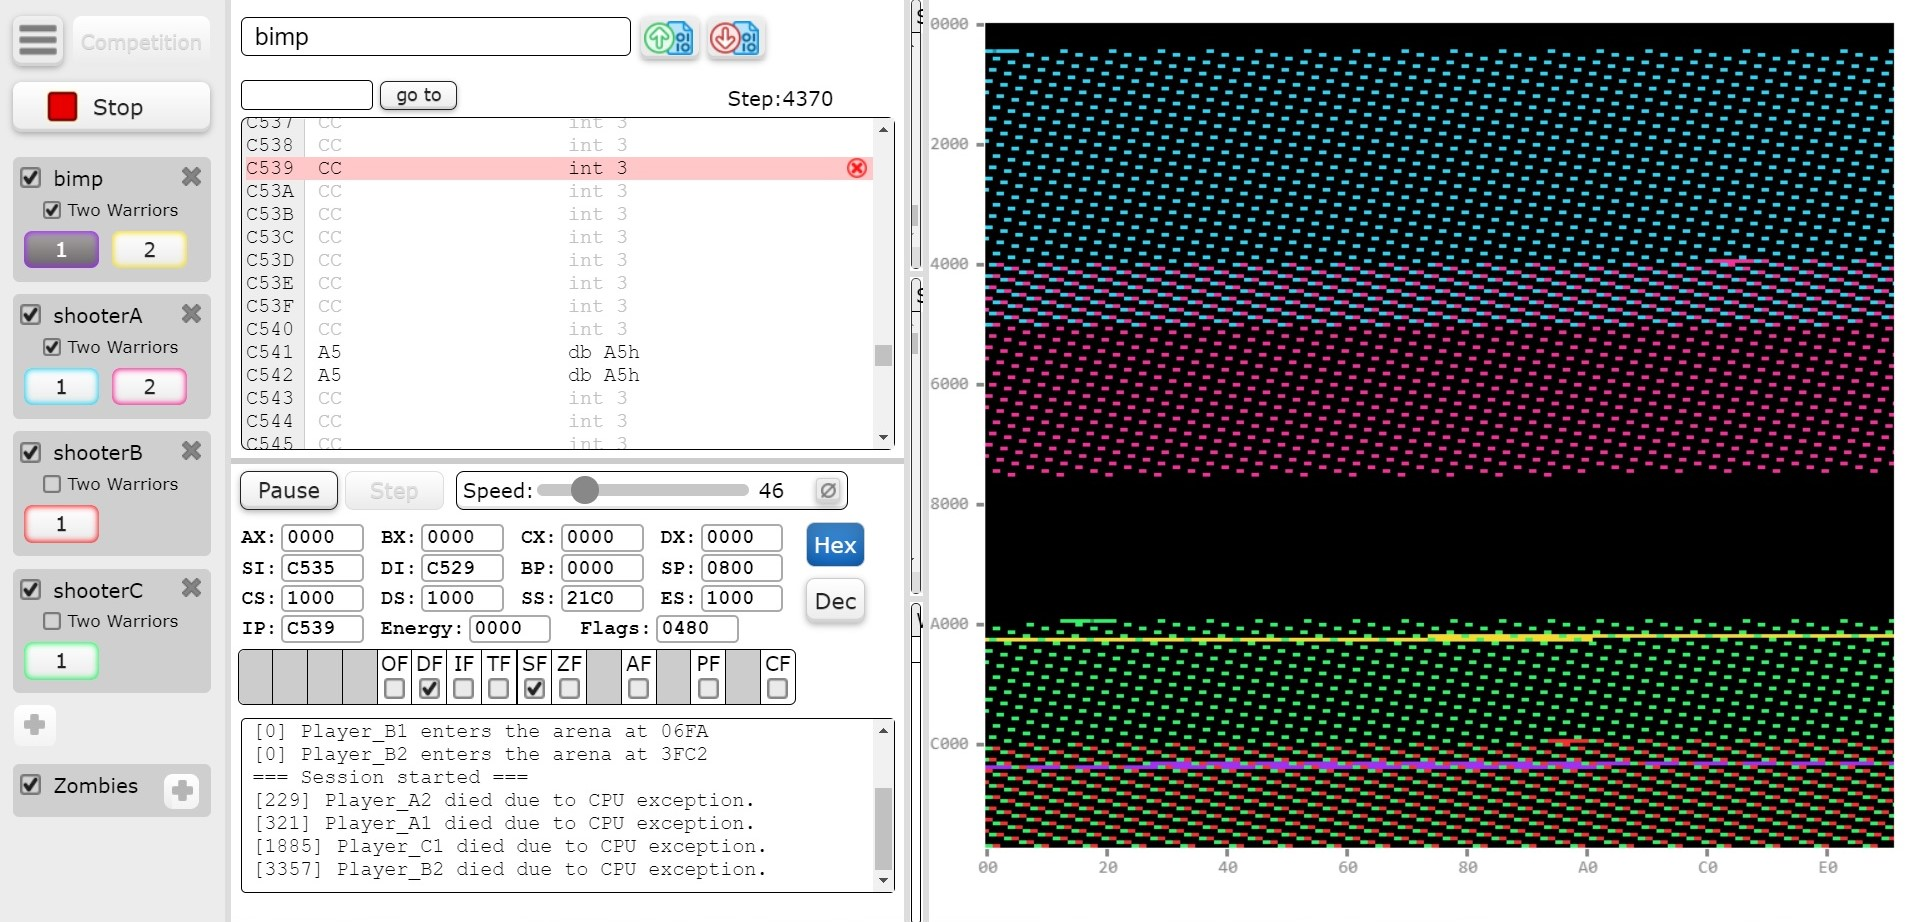
\includegraphics[width=\linewidth]{images/memory_use.jpg}
%     \caption{Memory arena}
%     \label{fig:image2}
%   \end{subfigure}
%   \caption{CodeGuru game}
%   \label{fig:CodeGuru-full}
% \end{figure}

\section{Method}
To evolve our survivors, we use Grammar-Guided Genetic Programming (G3P)---a technique that incorporates Genetic Programming principles, employs context-free grammar, often in a BNF form, and operates directly with tree-based representations. G3P allows evolving assembly programs following grammar type constraints and a defined aim, overtaking adversary in this case. During the evolutionary process with G3P, the evolved code is represented using an AST based on matching assembly BNF representation. 

% We evolved survivors to find weaknesses in past years' top survivors. 
% In each evolutionary experiment, we evolved survivors against one of the winning human-written survivors of past years' competition. As elaborated in \autoref{sec:results}, our evolved survivors were able to find weaknesses in most of them.
We now elaborate on the different parts of the evolutionary process.

\subsection{Representation}
Each individual consists of \textit{two} programs, called \textit{parts} (see \autoref{sec:codeguru}), represented by an AST. The AST follows a grammar defined by a BNF---a meta-syntax notation for context-free grammar consisting of derivation rules. Since assembly is a symbolic programming language, it can be represented using it. The terminals are opcodes and operands, and the functions are structures in the language (see listings \ref{tab:1_terminal_set} and \ref{tab:t2_function_set} in the appendix). We defined our types and derivation rules based on assembly language constraints. For example, we defined an unary command as a command consisting of an opcode that takes only one operand. Notably, except for a few CodeGuru special operators, our BNF is general and can match any 8086 assembly code. There are assembly commands that are not supported by the game's engine and were left out of the grammar to preserve legal programs.

\subsection{Evaluation}
\label{Evaluation_method}
% \cite{ModifiedEngine}
We evaluated survivors in each fitness calculation (in each generation) by running a CodeGuru game of 200 battles with the selected human-written survivor the evolution performed against. The game's engine is an open-source Java program that outputs the final scores for each game. As previously explained, the score is one point given to the last survivor alive. If several survivors stay alive, the point is divided equally between all. We modified the engine to produce more information about each game, as elaborated by the fitness function that has four parts:

\textit{Engine score:} the survivor's average engine score in all played games. 
\begin{center}
$f_{\text{score}} = \frac{\sum_{i=1}^{\text{games}} \text{score}_i}{\text{games}}$
\end{center}

\textit{Lifetime:} the normalized average number of rounds the survivor stayed alive.
\begin{center}
$f_{\text{lifetime}} = 0.1 \log_{10} max\left(1, \frac{\sum_{i=1}^{\text{games}} \text{reached\_round}_i}{\text{games}}\right)$
\end{center}

\textit{Written bytes:} the normalized average number of new bytes the survivor wrote. That is, the writing was performed on a memory fragment, which was not written before, or that the last one to write in was not the survivor itself.
\begin{center}
$f_{\text{written\_bytes}} = 0.1 \log_{10} max\left(1, \frac{\sum_{i=1}^{\text{games}} \text{written\_bytes}_i}{\text{games}}\right)$
\end{center}

\textit{Writing rate:} the average writing rate of the survivor.
\begin{center}
$f_{\text{writing\_rate}} = 0.1 \frac{\sum_{i=1}^{\text{games}} \text{written\_bytes}_i}{max\left(1, \sum_{i=1}^{\text{games}} \text{reached\_round}_i\right)} \times \frac{1}{\text{games}}$
\end{center}

The first two parts encourage evolution to win the competitions and survive for longer periods (respectively). The last two parts encourage the evolution of programs that write in different memory places, which enhances the chance of damaging opponents. We refer to the score parameter as the most significant since it reflects the performance compared to the adversary. Nevertheless, the other parts are important for guiding the evolution towards the different sub-goals and discriminating the individuals. Division by 10 and $\log_{10}$ were used on the original values of lifetime and written\_bytes in order to normalize them to an easy-to-process range yet maintain the tendency they represent. We also defined a bloat weight parameter, which equals $10^{-5}$. It slightly lowers the fitness of large evolved trees in order to prevent trees from bloating and yet allows large but powerful trees to evolve.

The fitness formula which performed the best was: 
\begin{equation*}
\begin{split}
  f = 2 f_{\text{score}} + 0.2 f_{\text{lifetime}} + 0.3 f_{\text{written\_bytes}} + 0.1 f_{\text{writing\_rate}} \\ - 10^{-5} max(\#part1\_nodes, \#part2\_nodes)  
\end{split}
\end{equation*}

It produces fitness values in the range of $[0, 2.5]$, which does not produce sharp deviations.
The chosen weights reflect the above-elaborated goals. The score is doubled due to its significance, resulting in a value in the range of $[0, 2]$. The additional parameters were multiplied by weights resulting in a mutual sum of $0.5$ at most, in order not to overshadow the score. According to conducted experiments, the writing\_rate parameter resulted in the smallest survivor's improvement, thus receiving the lowest weight. The experiments also showed the evolution was often able to independently learn the importance of the survivor's lifetime, on the contrary to the importance of performed writings, which it learned seldom. Thus, high and medium weights were given to written\_bytes and lifetime parameters respectively, to accelerate the improvement process.

\subsection{Genetic Operators}
\label{sec:method:operators}
We used Koza's standard mutation and crossover operators~\cite{koza1994genetic} that operate on the survivors' parts, which are represented as trees.
Specifically, we used the grow sub-tree (\ie sub-part) mutation and the exchange sub-tree (sub-part) crossover.
We added two more operators. The \textit{duplicate-tree} (part) mutation takes the best tree (part) of a survivor and replaces the second part with it. The \textit{exchange-trees} (parts) crossover replaces one of the trees (parts) of the first individual with one of the trees (parts) of the second.

\section{Experiments and Results}
\label{sec:results}
We carried out a comprehensive set of experiments aimed at winning the top human-written survivors. Our code is written in Python, using the EC-KitY toolkit~\cite{Sipper2023ECKity}. Our code and data are at~\href{https://github.com/irenamal/EC-KitY/tree/assembly_code_generation}{Assembly code generation}. 
% TODO: replace URL with the correct one.
The code for the human-written survivors we compete with can be found at~\cite{codeguru_repo}.

Experiments were conducted on a shared cluster of 96 nodes and a total of 5,408 CPUs (the most powerful processors are AMD EPYC 7702P 64-core, although most have lesser specs). 64 CPUs and 150 GB RAM were allocated for each evolutionary run (against one human adversary) to parallelize the evaluation. In practice, each run took approximately two days. 

The specific hyperparameters utilized in the experiments and their chosen values are detailed in \autoref{tab:hyperparameters}. The population size was chosen to be 192 to optimize the need for diversity, considering the resources of 64 CPUs and assigned time per evolutionary run. The Grow mutation probability was chosen to be 0.7 as the experiments that were conducted showed a clear tendency to better results with a high mutation rate, yet this rate allows evolution to perform a significant learning process. 

\begin{table}
\caption{Evolutionary hyper-parameters.}
\label{tab:hyperparameters}
\centering
\begin{threeparttable}
\renewcommand{\arraystretch}{1.3}
\begin{tabular}[t]{R{95px}|p{125px}}
Representation & Grammar-based GP \\
Mutation & Grow sub-tree and duplicate tree \tnote{$\dagger$} \\
Recombination & Exchange of sub-trees and trees \tnote{$\dagger$} \\
Grow mutation probability & 0.7\\
Duplication mutation probability & 0.2\\
Exchange sub-tree recombination probability & 0.3\\
Replacement recombination probability & 0.2\\
Parent selection & Tournament with $k=4$\\
Survivor selection & Generational replacement\\
Population size & 192\\
Termination & 2,000 generations or convergence with a winning strike
\end{tabular}
\renewcommand{\arraystretch}{1}
\begin{tablenotes}
\item[$\dagger$] The operators are described in \autoref{sec:method:operators}.
\end{tablenotes}
\end{threeparttable}
\end{table}

The operators were sequentially applied to individuals with different probabilities (\autoref{tab:hyperparameters}). 
The evolution was set to terminate when 2,000 generations are reached, or before, depending on whether convergence between best and average fitness values is achieved in addition to a monotonic non-increasing winning strike of 200 generations.

We repeated each experiment ten times to prove consistency. Our individuals' average fitness and standard deviation against each of the past years' winners are in \autoref{table:test_results}. We consider an average engine score higher than 0.5 a winning result for our individual. Notably, evolution managed to evolve assembly programs, which won almost 78\% of past years' human-written winners.

In the following sections, we inspect the code of the evolved solvers. The inspection revealed that the evolved survivors managed to win complex and long survivors using a relatively small code fragment. Although GP frequently evolves long code, sometimes only a small part of it is used in the program run flow and yet manages to win. As we will demonstrate, this shows how evolution found the Achilles' heel in the opponents' code and utilized it for its benefit.

\begin{table}
\caption{Test average fitness and standard deviation over ten experiments of our best individuals against past years' winners. }
\label{table:test_results}
\centering
\begin{tabular}{c|c|c|C{40px}|c} 
\toprule
\textbf{Year} & \textbf{Human survivor} & \textbf{\#Wins} & \textbf{Avg. Engine's Score} & \textbf{SD} \\
\midrule
2006 & Zeus & 8/10 & 0.675 & 0.162 \\
2007 & HutsHuts & 10/10 & 0.960 & 0.048 \\
2008 & APOCALYPSE & 9/10 & 0.741 & 0.170 \\
2009 & XLII & 9/10 & 0.891 & 0.174 \\
2010 & FSM & 3/10 & 0.481 & 0.147 \\
2011 & Mamaliga & 9/10 & 0.738 & 0.132 \\
2012 & Zorg & 9/10 & 0.692 & 0.171 \\
2013 & Snake & 10/10 & 0.736 & 0.136 \\
2014 & IamAA & 6/10 & 0.478 & 0.220 \\
2014 & Paranoia & 9/10 & 0.890 & 0.190 \\
2015 & SilentError & 9/10 & 0.684 & 0.127 \\
2016 & LoudBugFix & 2/10 & 0.402 & 0.078 \\
2017 & Memz & 10/10 & 0.997 & 0.006 \\
2018 & Barvaz'sAngles & 10/10 & 0.991 & 0.008 \\
2019 & Nuki'sDemons & 5/10 & 0.666 & 0.286 \\
2020 & GreeniEs & 10/10 & 0.984 & 0.020 \\
2021 & BlocksOfGuru & 10/10 & 0.753 & 0.118 \\
2022 & TheHeapMen & 4/10 & 0.494 & 0.102 \\
\bottomrule
\end{tabular}
\end{table}

\begin{figure*}
\captionsetup{type=lstlisting}
\centering
\begin{sublstlisting}{0.45\textwidth}
\begin{lstlisting}
@start:
and cl, [bx + 0x68 + 0x104 + 0x246]
div WORD [bx]
l8293849:
rcl dl, cl
rcl ax, 1
rol si, cl
push WORD [si]
shl dh, cl
l8293850:
and WORD [di + 0x222], 0x92
wait
wait
!\textcolor{red}{\textbf{mov WORD} [di], 0x196}!
jns l8293850
@end:
\end{lstlisting}
\caption{Part 1}
\end{sublstlisting}
\hfill
\begin{sublstlisting}{0.45\textwidth}
\begin{lstlisting}
@start:
sub bh, [bx + 0x30 + @start]
div WORD [bx]
l8293858:
rol dl, cl
shr di, 1
!\sout{dw 0x144}! inc sp
!\sout{push ds}! add [0xDA80], bx
!\sout{sbb dl, 0x34}! xor al, 0xD3
!\sout{sar ax, cl}! clc
l8293859:
and WORD [si + 0x246 + 0x230], 0x264
push bx
!\textcolor{red}{\textbf{pop WORD} [di]}!
and WORD [si + 0x206 + 0x202 + 0x220 + 0x-14 + 0x-20 + 0x32], 0x144
jmp l8293859
@end:
\end{lstlisting}
\caption{Part 2}
\end{sublstlisting}
\caption{Evolved survivor against Zorg (2012 winner). The two parts of the evolved survivor utilized Zorg's Achilles' heel by writing data to a part of its program. Strike-through text denotes run-time changed code.}
\label{evolved_zorg}
\Description{Code samples of the evolved survivor against Zorg (2012 winner). The two parts of the evolved survivor utilized Zorg's Achilles' heel by writing data to a part of its program.}
\end{figure*}

\subsection{Qualitative Analysis of Evolved Survivors}
\subsubsection{Utilizing Achilles' heel}
One of the clearest examples is Zorg---the 2012 winner. Zorg writes an important code fragment for its future run on memory address zero. The evolution process noticed it in about 100 generations and overridden this memory by addressing \lstin{di}, which holds the value zero, depriving Zorg of winning (see line 14 in both parts of \autoref{evolved_zorg}, which includes the dw translation to assembly commands and the effect on the following commands). Zorg's code is significantly longer and more complicated than the evolved fragment that overtook it. The evolved survivor manages to win Zorg in about 70\% of the battles in a game (according to the average engine's score) despite the weakness finding due to the randomness in the game's execution order.

\subsubsection{Concentrated vs. Scattered Memory Writes}
\label{scattered}
During evolution, we noticed several spikes in the best fitness. For example, when training against BlocksOfGuru, there were spikes in the fitness of the best individuals in generations 206 and 256 (see \autoref{fig:hist1}). To analyze these spikes, we ran a game with BlocksOfGuru against these individuals and the overall best individual (from generation 1,769). The results and memory image are depicted in \autoref{fig:joinedgame}.
We can see that most memory writes were made by the second part of the 1,769 and 256 individuals that cover the arena with scattered green and pink dots. 206's second part performed less, yet a significant number of writes in yellow are concentrated in several areas. All of the first part performed little to no new memory writes. Inspecting their cleared runnable code (Listings \ref{lst:BlocksOfGuru:a} and \ref{lst:BlocksOfGuru:b}) reveals that the first parts of 256 and 1,769 run in the loop written in their bottom, which keeps the individual alive but does not perform attacking actions---as seen in the lack of their color in the arena. In 206, both parts run in a loop due to \lstin{jmp ax} at the end, which jumps into the beginning of the code. Most memory writes of all individuals are performed using addressing \lstin{si}, yet with adding different constants to \lstin{si}. 256 and 1,769 use special constants like 65,535 and @start, while 206 does not. The first two exceed the bounds of word data, and the computation is thus written to an address defined as the special constant modulo $2^{16}$, which results in scattered writes. The evolutionary process discovered that scattered writing has more chances to encounter adversary code, as reflected in their higher scores, and it is reflected in runs against other survivors as well. 

\begin{figure}
    \centering
    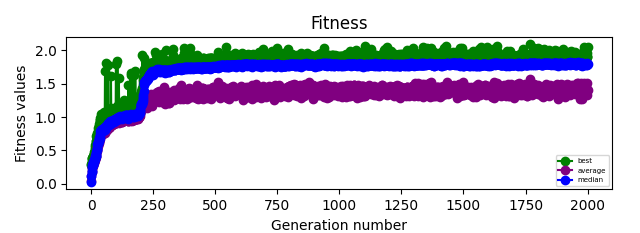
\includegraphics[width=\linewidth]{images/blocksofguru_hist_clipped.png}
    \caption{BlocksOfGuru (2021)}
    \label{fig:hist1}
    \Description{The graph describes best, median and average scores in each generation of the evolution. All the values converged starting from generation 300. While the best and median values are close, the average values are lower.}
\end{figure}

\begin{figure}
  \centering
    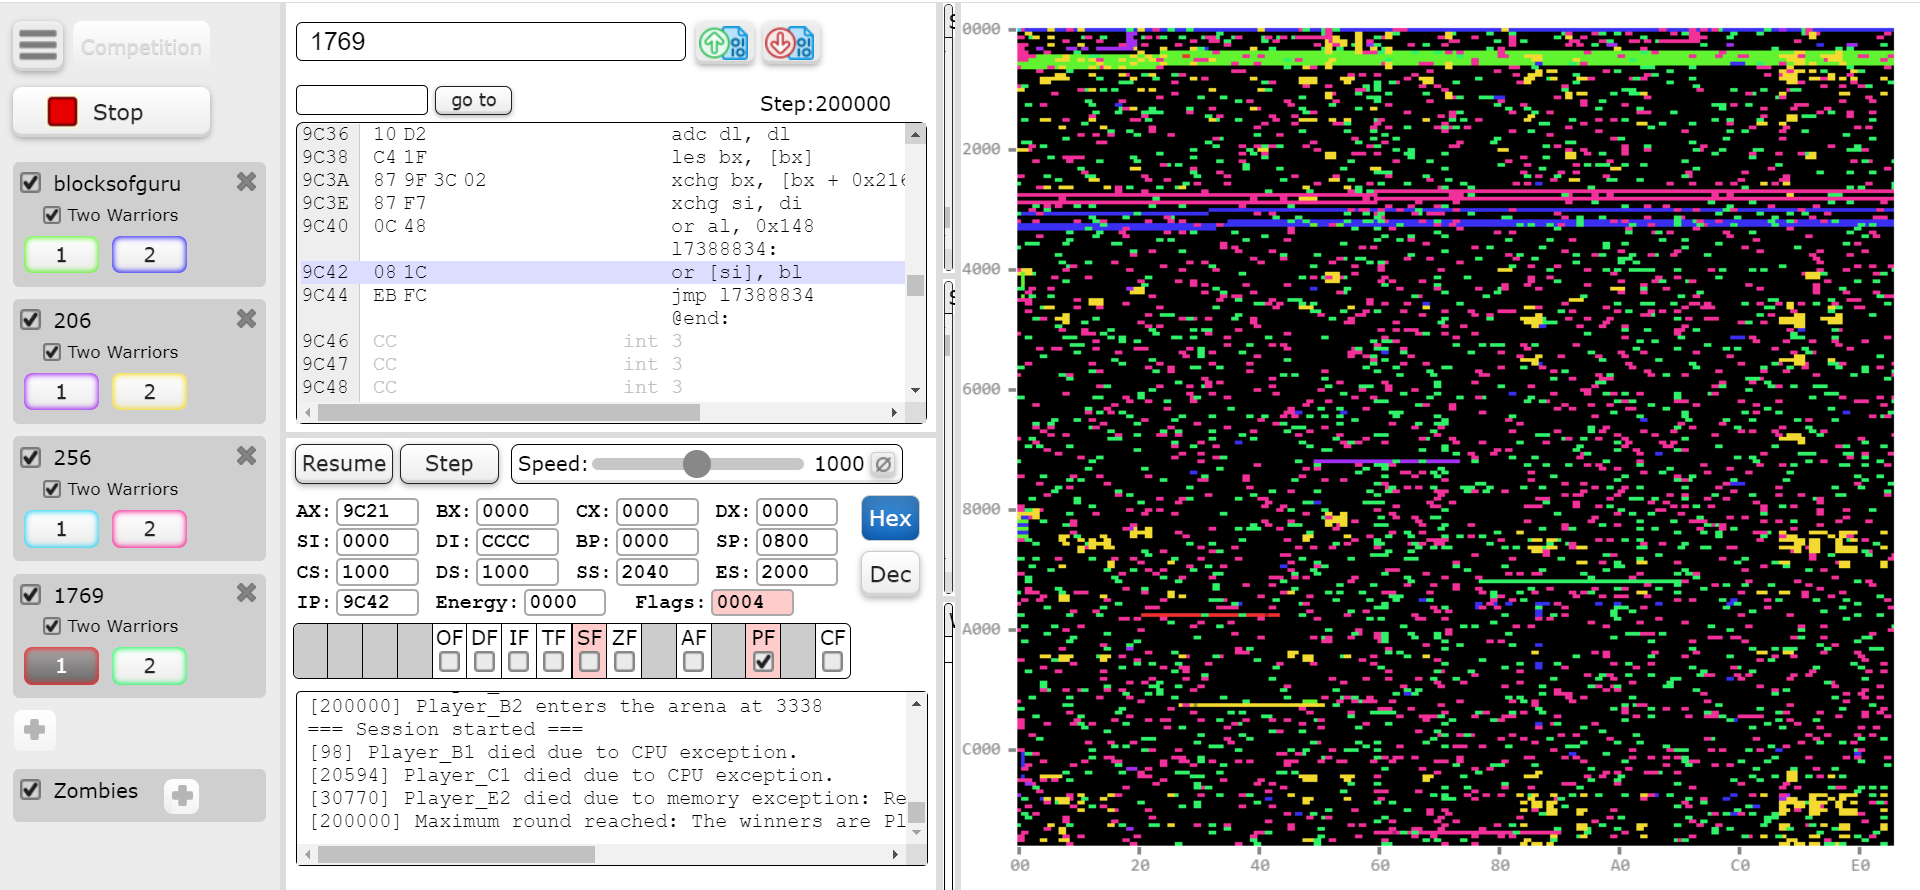
\includegraphics[width=\linewidth]{images/blocksofguru_generations_comparison_memory.png}
  \caption{The memory image of BlocksOfGuru vs. best individuals from generations 206, 256, and 1,769. The scattered green and pink dots are memory bytes written by the 1,769 and 256 individuals, respectively. The concentrated yellow dots are memory bytes written by 206 individual.}
  \label{fig:joinedgame}
  \Description{The memory image of BlocksOfGuru vs. best individuals from generations 206, 256, and 1,769. The scattered green and pink dots are memory bytes written by the 1,769 and 256 individuals, respectively. The concentrated yellow dots are memory bytes written by 206 individual.}
\end{figure}

\begin{figure*}
  \centering
  \begin{subfigure}{0.45\textwidth}
    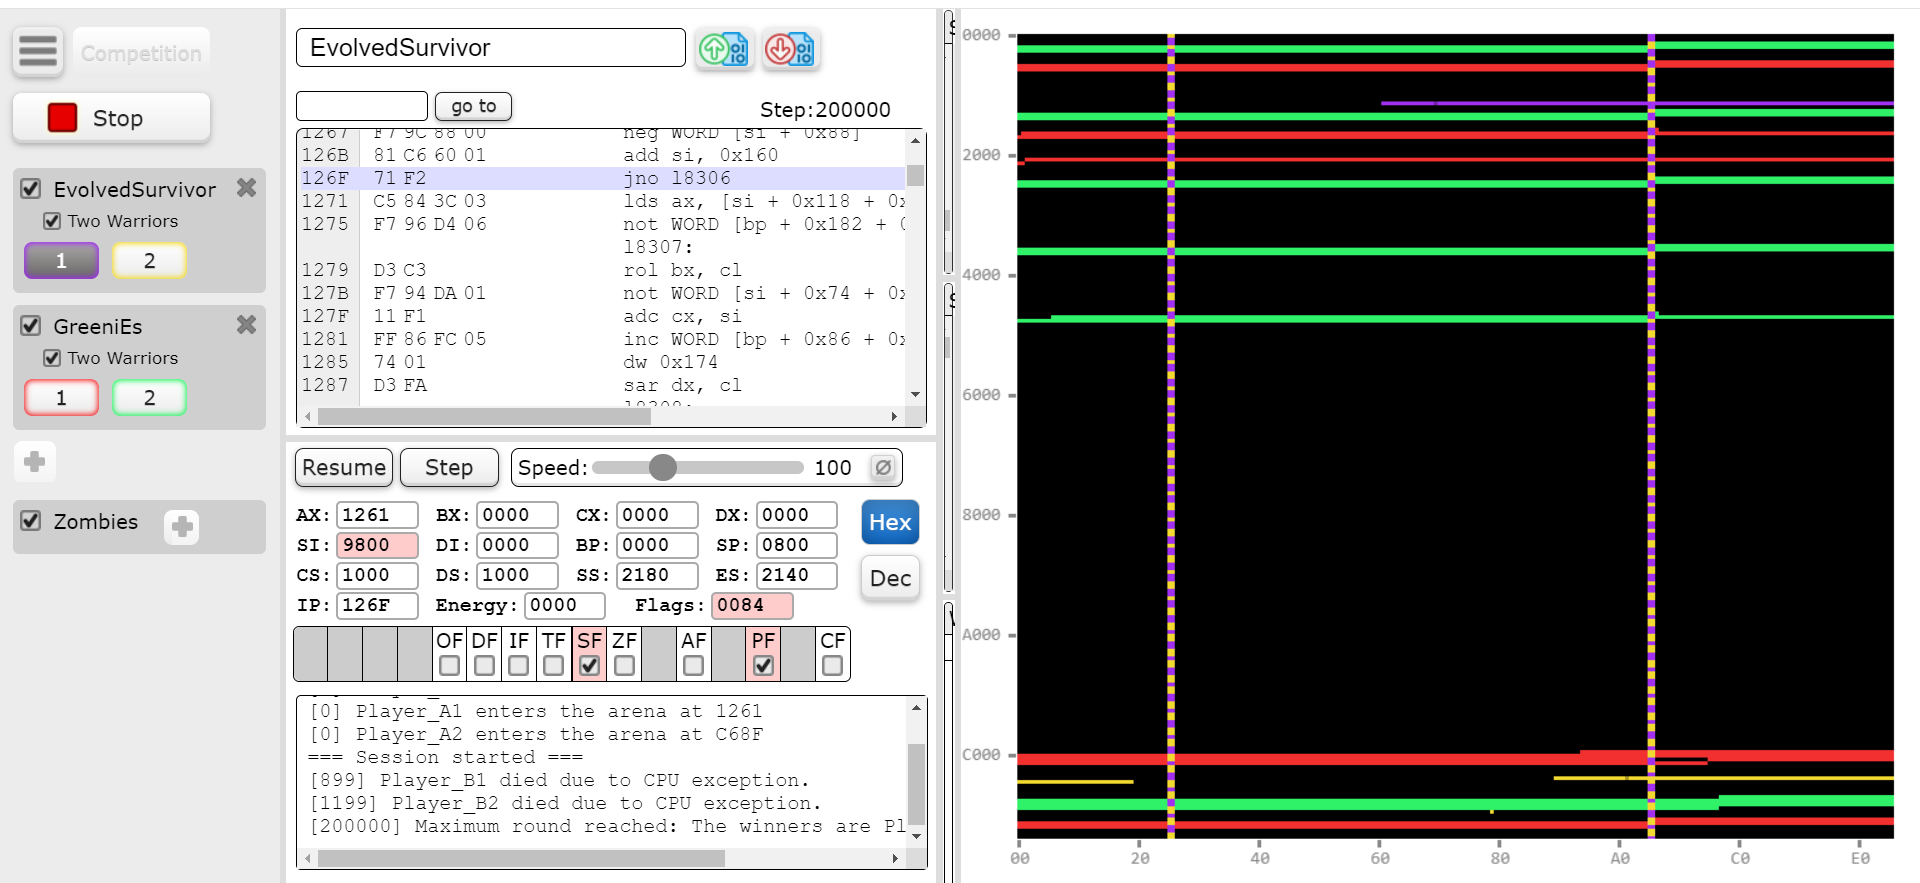
\includegraphics[width=\linewidth]{images/Greenies_vertical.png}
    \caption{Evolution vs. GreeniEs (2020)}
    \label{fig:mem_after2}
  \end{subfigure}
  \hfill
  \begin{subfigure}{0.45\textwidth}
    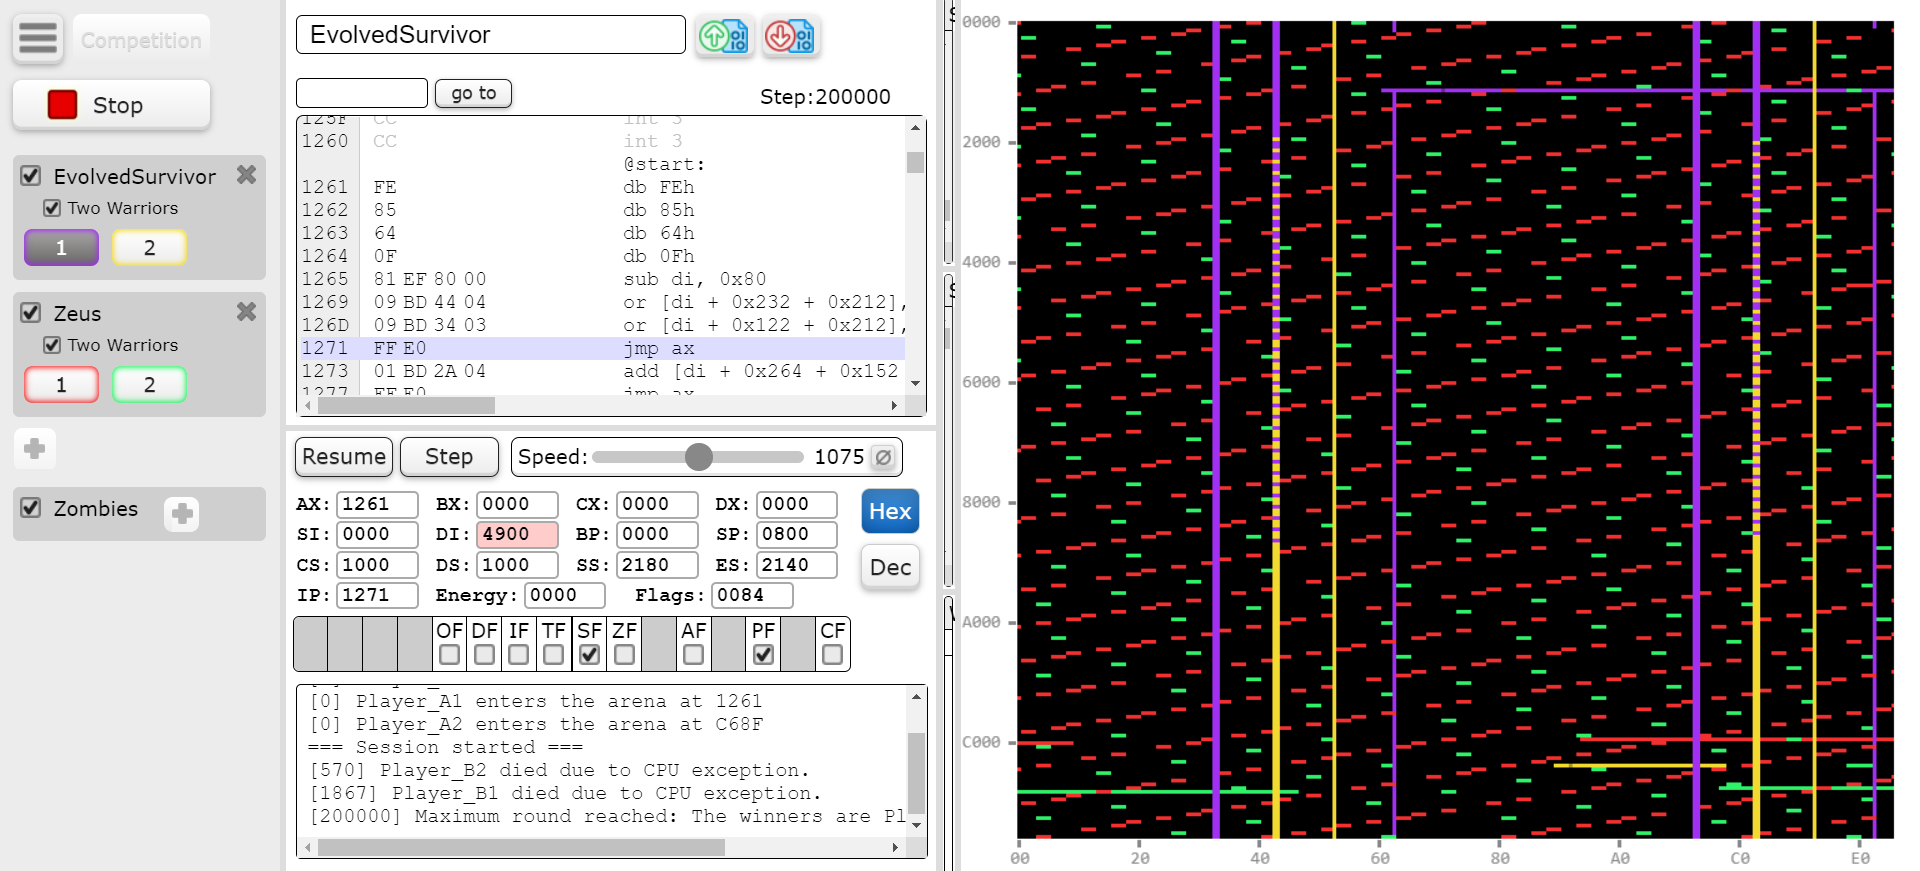
\includegraphics[width=\linewidth]{images/zeus_after_mem.png}
    \caption{Evolution vs. Zeus (2006)}
    \label{fig:mem_after1}
  \end{subfigure}
  \caption{Vertical vs. horizontal memory write. Horizontal writings of evolved survivors (in purple and yellow) ``cut'' the human-written adversaries that write in horizontal lines (green and red) by writing on their code before they reach their code.}
  \label{fig:vertical}
  \Description{Two captures of the memory arena in battles of evolved survivors vs. their opponent, reflecting vertical and horizontal writing patterns.}
\end{figure*}

\begin{figure*}
\captionsetup{type=lstlisting}
\centering
\begin{sublstlisting}[b]{0.23\textwidth}
\begin{lstlisting}
@start:
not WORD [bx+65535]
cmc
and [si+0x252],di
xchg bx,[si+0x051E]
jnc l268089
l268089:
add [si+0x0802+65535],bx
sbb cl,0x-14
loop l268090
l268090:
mov [si+@start+0x03B4],cx
rcr si,1
and [si],ax
jmp ax
@end:
\end{lstlisting}
\caption{206 part 1}
\end{sublstlisting}
\hfill
\begin{sublstlisting}[b]{0.22\textwidth}
\begin{lstlisting}
@start:
inc WORD [bx+65535]
cmc
and [si+0x252],cx
xchg bx,[si+0x051E]
jnc l268094
l268094:
add [si+0x0814+65535],bx
sbb cl,0x124
loop l268095
l268095:
mov [si+0x152],cx
rcr si,1
and [si],ax
jmp ax
@end:
\end{lstlisting}
\caption{206 part 2}
\end{sublstlisting}
\hfill
\begin{sublstlisting}[b]{0.19\textwidth}
\begin{lstlisting}
@start:
dec WORD [bx+65535]
cmc
and [si+0x252],dx
xchg bx,[di+0x05FC]
l376145:
sub [si],cl
jmp l376145
@end:
\end{lstlisting}
\caption{256 part 1}
\end{sublstlisting}
\hfill
\begin{sublstlisting}[b]{0.24\textwidth}
\begin{lstlisting}
@start:
inc WORD [bx+0x260+65535]
cmc
and [si+0x252],di
xchg bx,[si+0x0802+65535]
jnc l376150
l376150:
add [si+0x0802+65535],bx
sbb cl,0x-14
loop l376151
l376151:
mov [si+@start+0x03B4],cx
rcr si,1
and [si],ax
jmp ax
@end:
\end{lstlisting}
\caption{256 part 2}
\end{sublstlisting}
\caption{Comparing the code of best individuals against the BlocksOfGuru survivor.}
\label{lst:BlocksOfGuru:a}
\Description{The code of two evolved survivors against the BlocksOfGuru survivor during evolutionary process. Each one consists of two parts which run in a loop and perform input/output operations on registers and memory.}
\end{figure*}

\begin{figure}
\captionsetup{type=lstlisting}
\centering
\begin{sublstlisting}[b]{0.38\linewidth}
\begin{lstlisting}
@start:
xchg bp,[bp+0x0130]
and [di+0x072C],dx
xchg di,[di+0x05FC]
l7388834:
or [si],bl
jmp l7388834
@end:
\end{lstlisting}
\caption{1,769 part 1}
\end{sublstlisting}
\qquad
\begin{sublstlisting}[b]{0.5\linewidth}
\begin{lstlisting}
@start:
inc WORD [bx+0x260+65535]
cli
and [si+0x252],di
xchg bx,[si+0x0802+65535]
jnc l7388849
l7388849:
add [si+0x0802+65535],bx
sbb cl,0x-14
loop l7388850
l7388850:
mov [si+@start+0x03B4],cx
rcr si,1
and [si],ax
jmp ax
@end:
\end{lstlisting}
\caption{1,769 part 2}
\end{sublstlisting}
\caption{Comparing the code of best individuals against the BlocksOfGuru survivor.}
\label{lst:BlocksOfGuru:b}
\Description{The code of the best evolved survivor against the BlocksOfGuru survivor. Consists of two parts which run in a loop and perform input/output operations on registers and memory.}
\end{figure}

\subsubsection{Vertical vs. Horizontal Memory Writes}
\label{vertical}
Another interesting pattern we detected in evolved survivors was writing vertical bytes into memory. That is, sequentially writing a byte every 256 bytes, creating a vertical line in the memory state. This contrasts with human-written survivors, who usually write memory in horizontal lines (consecutive bytes). As a result, the evolved survivors were able to ``cut'' the adversary by writing on its code before the adversary reached its code. This is depicted, for example, in the memory state of our evolved individuals against Zeus (2006) and GreeniEs (2020) (see \autoref{fig:vertical}). The evolved survivors, in purple and yellow, write their code in vertical lines, thus cutting their adversaries' horizontal writing (in red and green). Writing vertically assures reaching the opponent's code faster because most submitted survivors take advantage of the maximum allowed code size, thus filling at least one memory row entirely. Therefore, filling one or a few columns will be faster than filling complete rows. A similar pattern was found in a significant part of runs against other survivors.

The presented patterns of utilizing weak points, scattered and vertical writings are expressed in a significant part of the performed evolutionary runs against all the survivors, although not all the runs of each survivor have used the same pattern.

\subsubsection{Random Generator Pattern}
The original program had difficulties overtaking a few previous years' winners, specifically FSM 2010, IamAA 2014, LoudBugFix 2016, and TheHeapMen 2022, resulting in an average score lower than 0.5. We assumed that human-written survivors may use randomness to be unpredictable, while our BNF has no element of randomness. Thus, we decided to add Pseudo-Random Number Generator (PRNG) patterns to our BNF. We added Linear Congruential Generator (LCG) and XOR-Shift Generators implementation to our grammar as shown in \autoref{table3_random_set} and ran the evolution against the above adversaries again for ten runs each.

% The randomness helped to improve, overtaking only one of the four human-written survivors, LoudBugFix \autoref{tab:test_random_results}. The evolved winner had the random patterns as part of its unreachable code, which means that its evolution helped to add it, and then 
% a misfortune mutation deactivated it. We believe it helped the evolution process, even though the winning survivor does not actively use it. The result increased from 0.402 to ?.

As shown in \autoref{tab:test_random_results}, using randomness improved the number of games evolution won and the average score in 3/4 of the cases.
The majority of the best-evolved individuals contained at least one of the random patterns. However, in some, the pattern appears in an unreachable code segment or outside the loop, meaning it only executes once. We believe it helped the evolution process, even though the winning survivor does not actively use it.
The use of randomness enhanced the use of scattered writing patterns (see \autoref{scattered}) for some of the survivors and evolved a combined horizontal-vertical writing pattern for others, in contrast to the described in \autoref{vertical}. The innovation the random pattern caused is the combination of the described patterns together, resulting in scattered writing in horizontal lines that expand vertically, as seen in \autoref{fig:fsm_rand}. We can see the yellow and purple memory cells that are being filled horizontally at the beginning. Afterward, the created lines expand vertically, and everything is done using scattered writing.   
%The randomness had the greatest affect on wining LoudBugFix (2016). 

\begin{table}
\centering
\begin{tabular}{c|c|C{20px}|C{25px}|C{20px}|C{25px}} 
\toprule
\multirow{2}{*}{\textbf{Year}} & \multirow{2}{*}{\textbf{Human Survivor}} & \multicolumn{2}{c|}{\textbf{w/o Random}} & \multicolumn{2}{c}{\textbf{w/ Random}} \\\cline{3-6}
&&\textbf{Avg. Score} & \textbf{\#Victories} & \textbf{Avg. Score} & \textbf{\#Victories} \\ 
\midrule
2010 & FSM & 0.481 & 3/10 & 0.483 & 5/10 \\
2014 & IamAA & 0.478 & 6/10 & 0.377 & 3/10 \\
2016 & LoudBugFix & 0.402 & 2/10 & 0.483 & 6/10 \\
2022 & TheHeapMen & 0.494 & 4/10 & 0.496 & 5/10 \\
\bottomrule
\end{tabular}
\caption{Test game result with and without randomness.}
\label{tab:test_random_results}
\end{table}

\begin{figure}
  \centering
    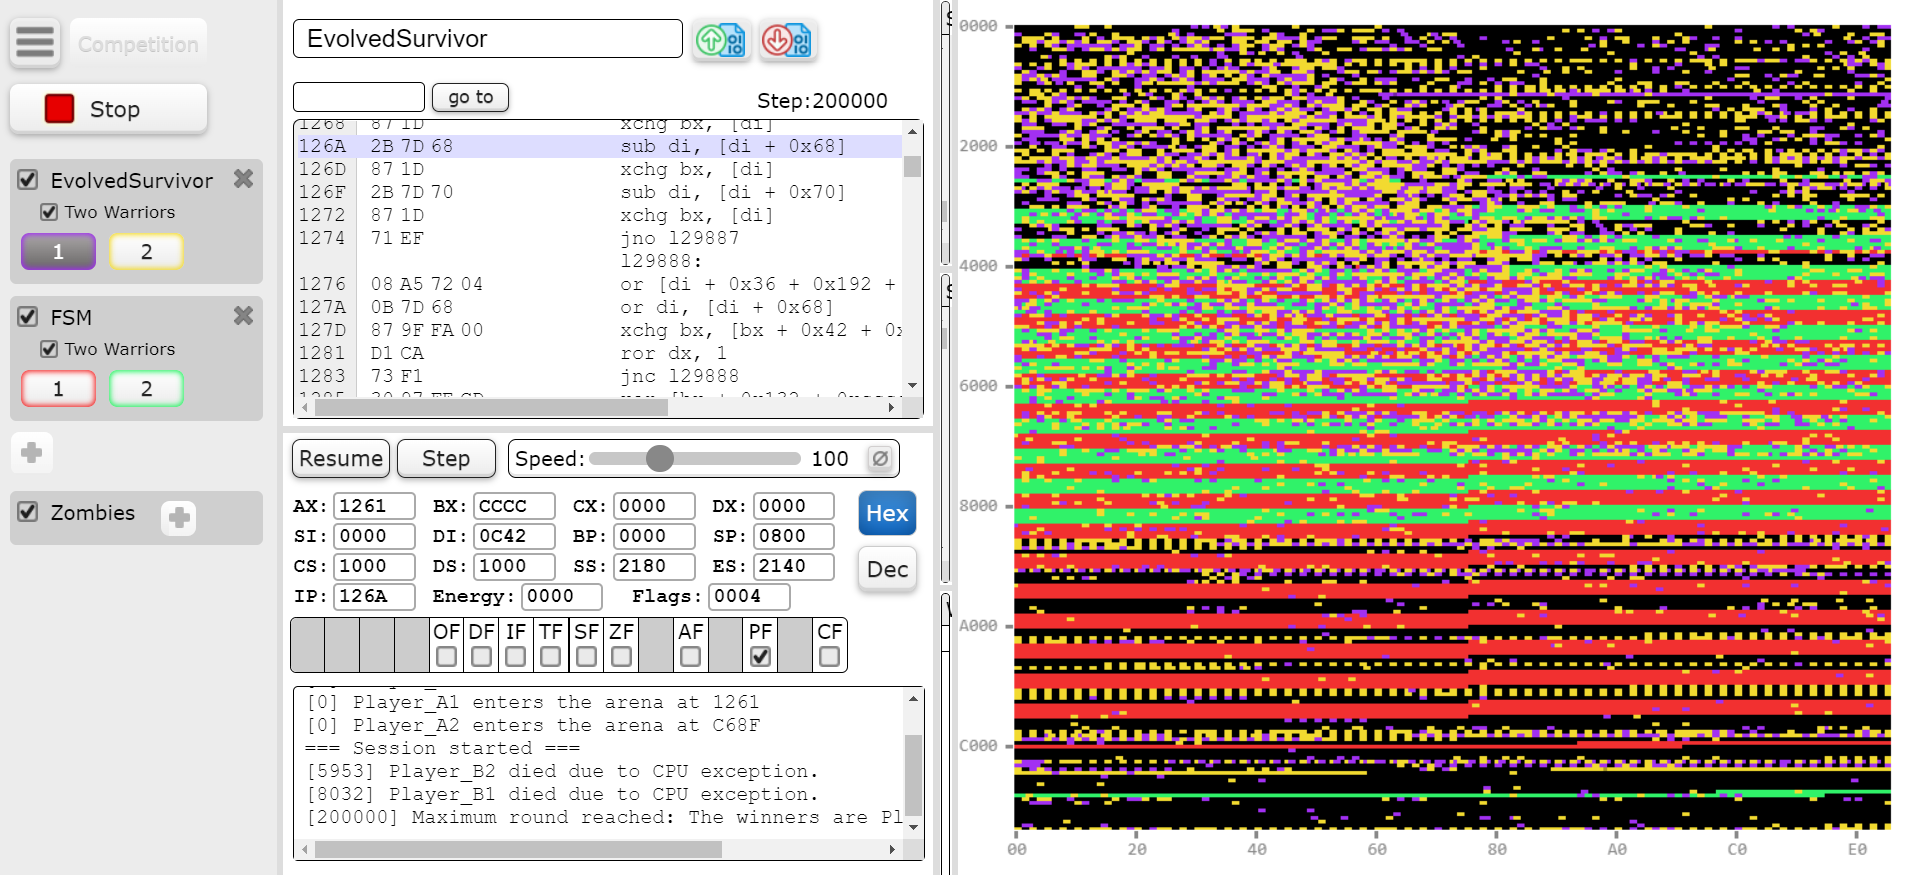
\includegraphics[width=\linewidth]{images/fsm_random.png}
    \caption{Scattered, horizontal, and vertical writing in the survivor which evolved using randomness patterns against FSM (2010).}
    \label{fig:fsm_rand}
    \Description{Capture of the memory arena reflecting scattered, horizontal, and vertical writing in the survivor which evolved using randomness patterns against FSM (2010).}
\end{figure}


%\newpage
%\subsection{Comparison to LLMs}
%\label{sec:llm}
%We compared our results to ChatGPT, one of today's leading LLMs. We explained the CodeGuru game, the special opcodes, and the rules using prompt engineering. We asked the chat for a survivor with the best chance to overtake others. The suggested code was tested against simple competition survivors that are given as examples in the game's web engine. At first, the provided survivors did not compile. After supplying corrections, they compiled; however, they achieved poor scores. Even when we supplied the opponents' code to ChatGPT, its produced survivor did not win. The prompts we used can be found at~\url{https://chat.openai.com/share/5ebda97c-06f8-4430-bd04-78a5abfc74ea}.
% Papailiopoulos~\cite{Mankowitz2023Faster} achieved the opposite result regarding Google's research. Faster sorting algorithms were discovered using deep reinforcement learning published. In his X account, he published ChatGPT-4 and achieved the same results in improving the code by removing the same command.

% These results show a primary success in the automatic evolution of assembly code from scratch in an adversarial environment. The results demonstrate G3P power to find a weakness in adversary code and utilize it to a defined goal. In our case, it was to win a CodeGuru game, however, any other goal can be defined through modifying the fitness calculation and minor grammar modifications.

% \subsection{Operators' Analysis}
% rs. We tested several mutation/crossover operators by performing a statistical analysis to evaluate their effectiveness over generations. We ran an evolutionary experiment where every five generations, we applied each operator $100$~times on the best individual and $100$~times on a random individual. All of the operators weakly improved the fitness of the best individual. However, the results on the random one showed an average improvement chance of about 50\% (depicted in \autoref{fig:Improvement_chance}).

% \begin{figure*}
%   \centering
%   \begin{subfigure}{0.45\textwidth}
%     \includegraphics[width=\linewidth]{images/refactored_crossover_improvment.png}
%     \caption{Exchange sub-trees crossover.}
%     \label{fig:cross}
%   \end{subfigure}
%   \hfill
%   \begin{subfigure}{0.45\textwidth}
%     \includegraphics[width=\linewidth]{images/refactored_replacing_improvement.png}
%     \caption{Exchange trees (parts) crossover.}
%     \label{fig:rep}
%   \end{subfigure}
  
%   \begin{subfigure}{0.45\textwidth}
%     \includegraphics[width=\linewidth]{images/refactored_muatation_improvement.png}
%     \caption{Grow sub-tree mutation.}
%     \label{fig:mut}
%   \end{subfigure}
%   \hfill
%   \begin{subfigure}{0.45\textwidth}
%     \includegraphics[width=\linewidth]{images/refactored_duplication_improvment.png}
%     \caption{Duplicate tree (part) mutation.}
%     \label{fig:dup}
%   \end{subfigure}
  
%   \caption{Genetic operators analysis. The graphs show the probability of improving a random individual's fitness over the generations with each operator.}
%   \label{fig:Improvement_chance}
% \end{figure*}

\section{Connection to Cyber Security}
Signatures are widely used in anti-virus programs as a technique to detect known malwares. Characterizing and unique features of the malware are joined together using matching functions, documented in various formats (\eg hashes, Yara) and are stored in databases to be further used to identify the malicious code fragments. The same function is calculated on each file scanned by the anti-virus and the result is compered to the documented ones. If there is an equality, than the malware exists in the document. If there isn't, it doesn't inevitably mean the file is safe, however the documented malwares are not found in it.  
To bypass those techniques, malware developers found ways to modify their code so it will not be recognized by the signatures and yet the functionality of the malware will be preserved, continuing the infinite protector-attacker struggle.

Assembly code evolution and CodeGuru serve as an interesting platform to analyze the ability of evolution to overcome tools designed especially against it, like the ability of malware developers to overcome signatures against the malwares.
As mentioned in \autoref{sec:codeguru}, there is a special opcode \texttt{INT 0x87} in the game. It looks for 4 byte sequence identical to the values stored in the registers AX:DX and replaces them with the values stored in BX:CX. The search is performed in the memory starting from address DI:ES moving up or down, determined by the direction flag. Therefore, if a command from a survivor is stored in AX:DX, it can be found and replaced by the adversary to an illegal command stored in BX:CX, causing the survivor to run it and be disqualified. This simulates the identification of a malware using a signature.

We performed an experience utilizing \texttt{INT 0x87} command to emulate signature based anti-virus. We chose XLII (2009) and GreeniEs (2020) as adversaries, two human-written survivors we previously overtook and which use \texttt{INT 0x87} in their code. Full evolutionary processes were performed against them, with a slight modification of intended several minutes pause when the evolved population reaches consistent win identified by average fitness of 1.1, which obligates a wining score (as elaborated in \autoref{Evaluation_method}). During this pause, we manually modified the AX:DX values the adversaries use with  \texttt{INT 0x87} to commands the best evolved individuals depend on and continued the evolution. This faced the evolved population with an adversary specially tailored against it.
As seen in \autoref{fig:antivirus}, in both cases, the fitness dropped in the following generation. As an expected outcome of facing improved adversary. However, as the evolution proceeded, it was able to even and improve the fitness results. 
The evolution succeeded to replaced the targeted commands by different ones with similar behavior.  
The results prove evolution can face tools designed especially against it. Combined with the fact the used grammar represents general assembly and the fact many malwares are written in assembly, these findings can be utilized to modify malwares in order to evade signature based anti-virus systems. 

\begin{figure*}
  \centering
  \begin{subfigure}{0.45\textwidth}
    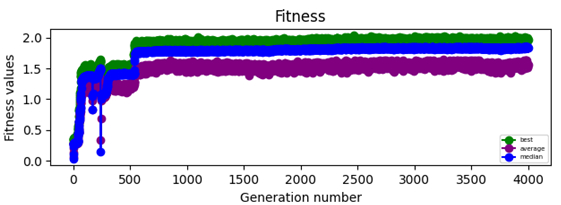
\includegraphics[width=\linewidth]{images/xlii_antivirus.png}
    \caption{Evolution vs. modified XLII (2009)}
    \label{fig:antivirus1}
  \end{subfigure}
  \hfill
  \begin{subfigure}{0.45\textwidth}
    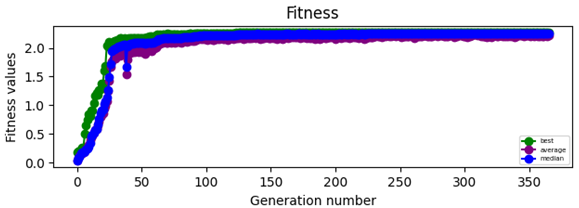
\includegraphics[width=\linewidth]{images/greenies_antivirus.png}
    \caption{Evolution vs. modified GreeniEs (2020)}
    \label{fig:antivirus2}
  \end{subfigure}
  \caption{The fitness dropped in generation 241 and 38 respectively after the "tailor made" adversary was created}
  \label{fig:antivirus}
  \Description{The fitness dropped in generation 241 and 38 respectively after the "tailor made" adversary was created}
\end{figure*}


\section{Conclusion}
This work presented the evolution of assembly code from scratch in an adversarial environment, specifically the CodeGuru Xtreme competition. Through the use of GP, we synthesized assembly code that outperformed human-written winning survivors from past years. Our evolved programs were able to identify and exploit weaknesses in the programs they were trained against. %Additionally, we compared our approach with the use of a Large-Language Model (LLM) and demonstrated that the LLM was unable to generate a survivor capable of winning any competition.

CodeGuru Xtreme competition serves as a valuable platform for studying GP and code evolution in adversarial environments. To facilitate further research in this direction, we have provided a comprehensive qualitative analysis of the evolved survivors and the weaknesses they have identified. While we were able to overtake most of the top human-written survivors, the domain is far from being solved. There are still some survivors that evolution failed to win, and the evolved survivors were only able to win against one survivor at a time.

The implications of this work extend beyond the CodeGuru Xtreme competition. Utilizing evolution to detect weaknesses in other survivors has important applications in cyber-security. Furthermore, the assembly language used in this research is also relevant in the context of computer viruses. We believe that by modifying the fitness function, our approach can be employed to identify weaknesses in code and aid in their resolution.

\newpage
%\balance
\bibliographystyle{ACM-Reference-Format}
\bibliography{references,achiya}  

\clearpage
\appendix

\section{Our Grammar}
\begin{BNF}
\begin{framed}
\begin{grammar}
<reg> ::= `ax', `bx', `cx', `dx', `si', `di', `bp', `sp' 

<half\_reg> ::= `ah', `al', `bh', `bl', `ch', `cl', `dh', `dl'

<addres> ::= `[bx]', `[si]', `[di]', `[bp]'

<pop\_reg> ::= `ax', `bx', `cx', `dx', `si', `di', `bp', `WORD [bx]', `WORD [si]', `WORD [di]', `WORD [bp]', `ds', `es'

<push\_reg> ::= `ax', `bx', `cx', `dx', `si', `di', `bp', `WORD [bx]', `WORD [si]', ` WORD [di]', ` WORD [bp]', `ds', `es', `cs', `ss'

<const> ::= [(2*i) for i in range(-10, 133)]', `@start', `@end', `65535', `0xcccc'

<op> ::= `nop', `stosw', `lodsw', `movsw', `cmpsw', `scasw', `pushf', `popf', `lahf', `stosb', `lodsb', `movsb', `cmpsb', `scasb', `xlat', `xlatb', `cwd', `cbw', `cmc', `clc', `stc', `cli', `sti', `cld', `std'

<op\_single> ::= `div', `mul', `inc', `dec', `not', `neg'

<op\_double> ::= `cmp', `mov', `add', `sub', `and', `or', `xor', `adc', `sbb', `test'

<op\_jmp> ::= `jmp', `jcxz', `je', `jne', `jp', `jnp', `jo', `jno', `jc', `jnc', `ja', `jna', `js', `jns', `jl', `jnl', `jle', `jnle', `loopnz', `loopne', `loopz', `loope', `loop'

<op\_rep> ::= `rep', `repe', `repz', `repne', `repnz'

<op\_function> ::= `call', `call near', `call far'

<op\_special> ::= `wait wait wait wait', `wait wait', `int 0x86', `int 0x87'

<op\_pointer> ::= `lea', `les', `lds'

<op\_ret> ::= `ret', `retn', `retf', `iret'

<op\_push> ::= `push'

<op\_pop> ::= `pop'

<op\_double\_no\_const> ::= `xchg'

<op\_shift> ::= `sal', `sar', `shl', `shr', `rol', `ror', `rcl', `rcr'

<section> ::= ` ' 
\end{grammar}
\end{framed}\vspace{-1em}
\caption{Terminals definitions}\vspace{2em}
\label{tab:1_terminal_set}
\end{BNF}
%\newpage

\begin{BNF}
\begin{framed}
\begin{grammar}
<section> ::= <label> <section> <backwards\_jump> <section>
\alt <label> <section> <backwards\_jump>
\alt <section> <forward\_jmp><section> <label> <section>
\alt <label> <section> <call\_func> <backwards\_jump> <label> <section> <return>
\alt <op\_double> <reg>  <reg | const | address> <section>
\alt <op\_double> <address> <reg | half\_reg> <section>
\alt <op\_double> <half\_reg> <half\_reg | const | address> <section>
\alt <op\_double> <WORD | BYTE> <address> <const> <section>
\alt <op\_pointer> <reg> <address> <section>
\alt <op\_double\_no\_const> <reg> <reg | address> <section>
\alt <op\_double\_no\_const> <half\_reg> <half\_reg | address> <section>
\alt <op\_single> <reg | half\_reg> <section>
\alt <op\_single> <WORD | BYTE> <address> <section>
\alt <op\_function> <address> <section>
\alt <op | op\_special> <section>
\alt <op\_rep> <op> <section>
\alt <op\_push> <push\_reg> <section>
\alt <op\_pop> <pop\_reg> <section>
\alt `jmp' <reg | address> <section>
\alt `dw 0x'<const> <section>
\alt <op\_shift> <reg | half\_reg> <cl | 1> <section>

<call\_func> ::= `call l'<const> <section>

<return> ::= <op\_ret> <section>

<label> ::= `l'<const> <section>

<forward\_jump> ::= <op\_jmp> `l'<const> <section>

<backwards\_jump> ::= <op\_jmp> `l'<const>`-1' <section>

<address> ::= [<address> + <const>] 
\end{grammar}
\end{framed}\vspace{-1em}
\caption{Functions definitions}\vspace{2em}
\label{tab:t2_function_set}
\end{BNF}

\begin{BNF}
\setlength{\grammarindent}{6em}
\begin{framed}
\begin{grammar}
<section> ::= mov ax, timestamp\\
mov <reg>, 1664525\\
mul <reg>\\
add ax, 1013904223 <section>

<section> ::= mov <reg>, randint(0, 65,535)\\
mov <reg>, randint(0, 65,535)\\
xor <reg>, <reg>\\
shl <reg>, 7\\
shr <reg>, 5\\
xor <reg>, <reg> <section>
\end{grammar}
\end{framed}\vspace{-1em}
\setlength{\grammarindent}{2em}
\caption{Functions definitions for the random patterns.}\vspace{2em}
\label{table3_random_set}
\end{BNF}

\end{document}
